\documentclass{article}
\usepackage{preamble}
\begin{document}
\title{Exploration in \GROOVE}
\author{Arend Rensink}
\date{August 2024}
\maketitle

\section*{Terminology}

The following is a list of properties of states and transitions, marked \textbf{S} and/or \text{T} to signify whether they apply to states, transitions or both. Figure~\ref{fig:venn} shows these different concepts in relation to each other.

\begin{description}
\item[Absence level (S)] The \emph{absence level} of a state is the minimal transience level of that state and all its transitive successors. It follows that the \emph{absence level} is smaller than or equal to the \emph{transience level}. As long as a state is not \emph{full}, its \emph{absence level} may decrease as a consequence of further exploration.

\item[Absent (S,T)] A state or transition is \emph{absent} if it should not be considered to be part of the state space. In particular, a state is \emph{absent} if it is \emph{full} and has positive \emph{absence level}; a transition is \emph{absent} if its source or target state is \emph{absent}. It follows that an \emph{absent} state is always \emph{transient}. Whether or not a state or transition is \emph{absent} is independent of whether or not it is \emph{inner}.

\item[Atomic (T)] A transition is \emph{atomic} if it is \emph{outer} and its source and target states are \emph{steady}.

\item[Closed (S)] A state is \emph{closed} if it is not \emph{open}. A \emph{closed} state may or may not be \emph{full}.

\item[Final (S)] A state is \emph{final} if exploration is considered to terminate after reaching it. For instance, if two control blocks are concatenated, the second comes into play after the exploration of the first has reached a final state; also, if a state space is wrapped in an atomic block, the only \emph{steady} states, apart from the \emph{initial} state, are the \emph{final} ones. In other words, \emph{final} has the typical meaning in (regular) automata. A \emph{final} state is certainly \emph{closed} and \emph{steady}; it may or may not have successors.

\item[Full (S)] A state is \emph{full} if it is \emph{closed} and all successors up to (but not necessarily including) the first \emph{steady} state are also \emph{closed}. This means that the status of the state is fully known; in particular, it is possible, on the basis of its successors, to decide whether the state is \emph{absent}.

\item[Initial (S)] A state is \emph{initial} if it is the start state for the exploration. Its \emph{prime} is \emph{steady}.

\item[Inner (S,T)] A state is \emph{inner} if it is inside the atomic block that makes up the body of a recipe, and a transition is \emph{inner} if it is a step in the execution of a recipe. Hence, an \emph{inner} state is certainly \emph{transient}, but the inverse does not hold. An \emph{inner} state that is not \emph{closed} may still evolve into an \emph{outer} one as a consequence of further exploration.

\item[Latent (S)] A state is \emph{latent} if it is neither \emph{present} nor \emph{absent}. Since \emph{full} states are always either \emph{present} or \emph{absent}, \emph{latent} are certainly \emph{short}.

\item[Open (S)] A state is \emph{open} if its direct outgoing transitions are not fully known. It follows that an open state can become \emph{closed} through further exploration of its outgoing transitions.

\item[Outer (S,T)] A state or transition is \emph{outer} if it is not \emph{inner}.

\item[Partial (T)] A transition is \emph{partial} if it is not \emph{atomic}, meaning that it is a proper (sub)part of an atomic block. These include \emph{inner} transitions that constitute single-step recipe executions.

\item[Present (S,T)] A state is \emph{present} if it has a transitive successor that is \emph{steady} (in other words, it has \emph{absence level} zero); a transition is \emph{present} if its source and target are \emph{present}. If a state is not \emph{present}, it is either \emph{latent} or \emph{absent}; if a transition is not \emph{present}, it is \emph{absent}.

\item[Prime (S)] The \emph{prime} of a state is the version of that state when it is just discovered, and no outgoing transitions have been explored. Hence, the \emph{prime} may be \emph{transient} even though (because of further exploration) the state itself has become \emph{steady} because its \emph{transience level} has decreased to zero.

\item[Private (S,T)] A state or transition is \emph{private} if it is not \emph{public}; in other words, if it is either \emph{inner} or \emph{absent}.

\item[Public (S,T)] A state or transition is \emph{public} if it is both \emph{outer} and \emph{present} (or, in other words, if it is neither \emph{inner} nor \emph{absent}).

\item[Short (S)] A state is \emph{short} if it is not \emph{full}.

\item[Steady (S)] A state is \emph{steady} if it is not \emph{transient}.

\item[Transience level (S)] The \emph{transience level} of a state is the number of (nested) atomic blocks that it is inside of. A state is \emph{steady} if and only if its \emph{transience level} is zero; otherwise it is \emph{transient}. As long as a state is not \emph{closed}, its \emph{transiene level} may decrease as a consequence of further exploration.

\item[Transient (S)] A state is \emph{transient} if it is inside an atomic block, meaning that it has a positive \emph{transience level}. A \emph{transient} state may or may not be \emph{inner}. A transient state that is \emph{open} may still evolve into a \emph{steady} state as a consequence of further exploration.
\end{description}

\begin{figure}
\centering
\begin{subfigure}{0.4\textwidth}
\centering
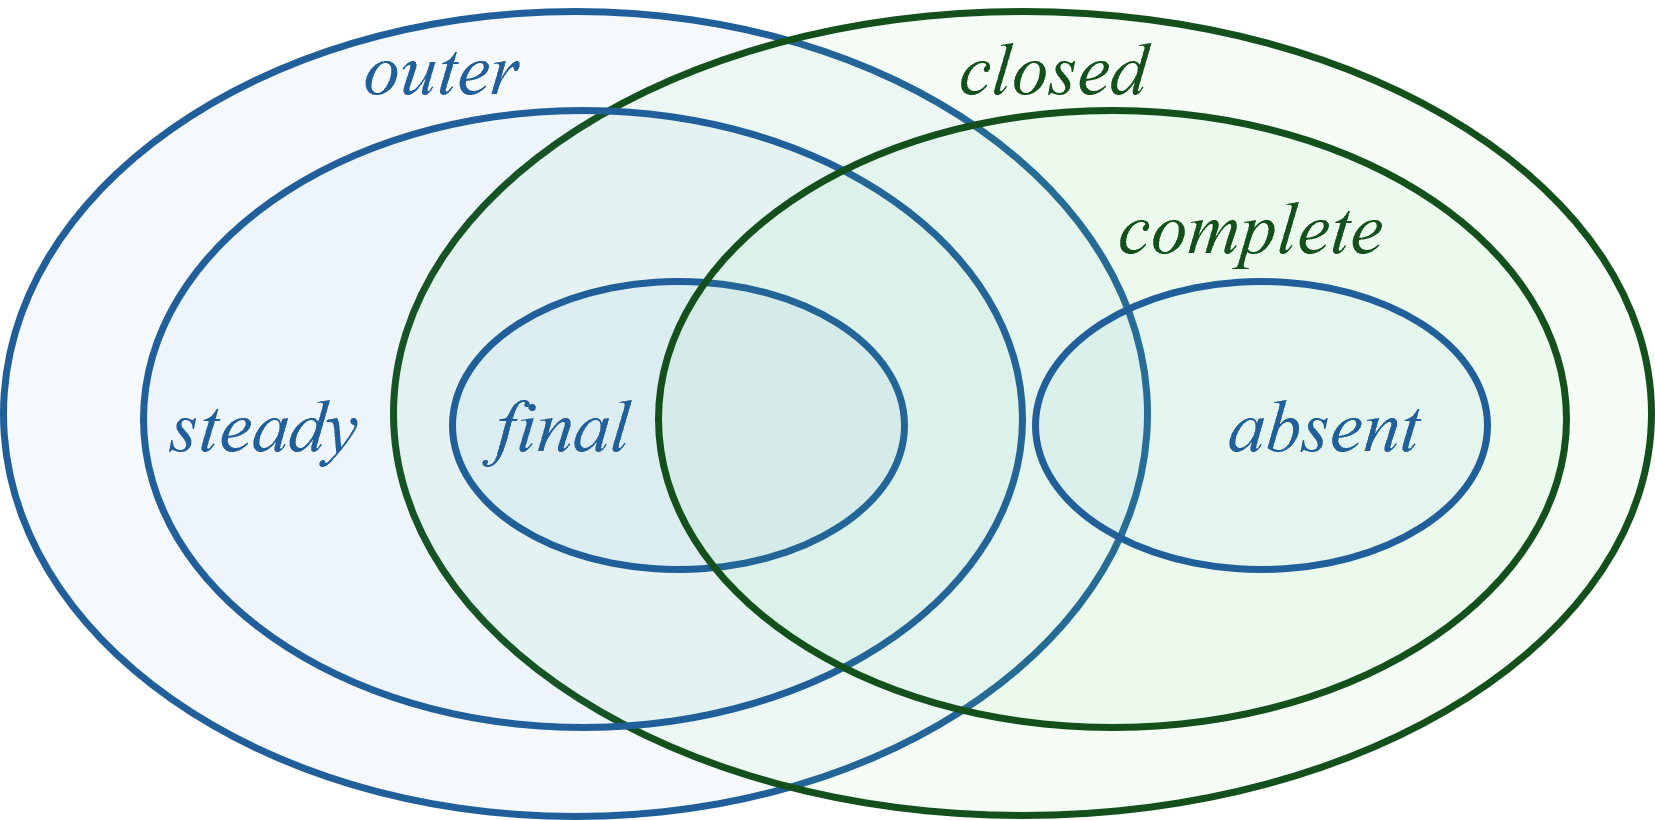
\includegraphics[scale=.4]{figs/s-venn}
\caption{States}
\end{subfigure}%
\begin{subfigure}{0.3\textwidth}
\centering
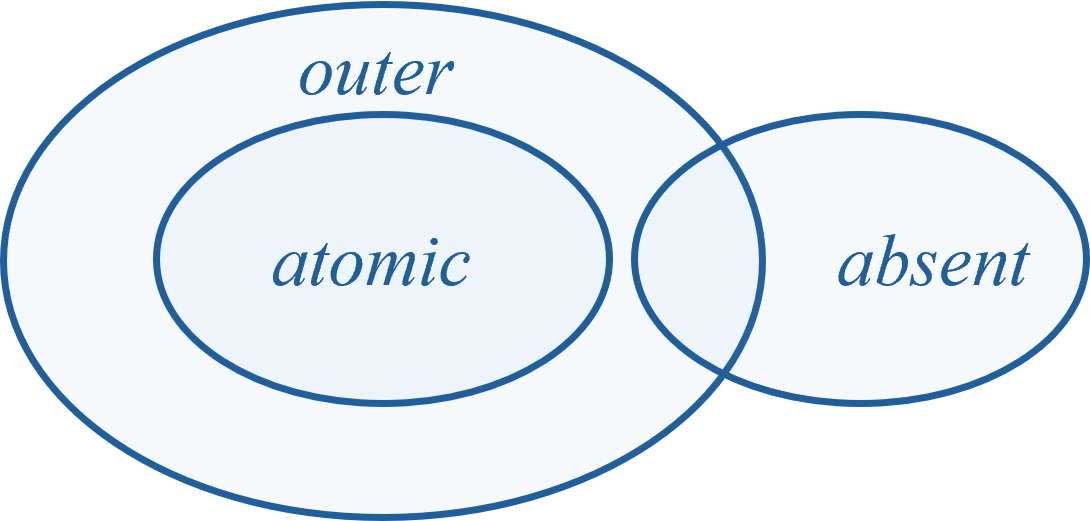
\includegraphics[scale=.4]{figs/t-venn}

\bigskip\bigskip
\caption{Transitions}
\end{subfigure}%
%
\begin{subfigure}{.25\textwidth}
\centering
\scalebox{.7}{$\begin{array}[b]{@{}r@{{\;\equiv\;}}l@{}}
\mathit{absent} & \mathit{full} \wedge \neg\mathit{present} \\
\mathit{inner} & \neg\mathit{outer} \\
\mathit{latent} & \neg\mathit{full} \wedge \neg \mathit{present} \\
\mathit{open} & \neg\mathit{closed} \\
\mathit{partial} & \neg\mathit{atomic} \\
\mathit{private} & \neg\mathit{public} \\
\mathit{public} & \mathit{outer} \wedge\mathit{present} \\
\mathit{short} & \neg\mathit{full} \\
\mathit{transient} & \neg\mathit{steady}
\end{array}$}

\bigskip\bigskip
\phantomcaption
\end{subfigure}
\caption{Properties of states and transitions}
\label{fig:venn}
\end{figure}


\section*{State spaces}

\medskip\noindent
We globally assume a set of labels $A$.

\medskip\noindent 
A \emph{state space fragment} is a tuple $\cS=\tupof{S,\Init,{\trans{}},{\final},\TLevel,\Closed}$ with
\begin{itemize}
\item $S$ a set of states;
\item $\Init\in S$ the initial state;
\item ${\trans{}}\subseteq S\times A\times S$ a transition relation;
\item ${\final}\subseteq S$ a termination predicate, such that $p\trans a q$ implies $\neg p\final$;
\item ${\TLevel}:S\to \natN$ a \emph{transience level} function, such that $\TLevel(\Init)=0$;
\item $\Closed\subseteq S$ a set of \emph{closed states}, such that $\final\subseteq \Closed$.
\end{itemize}
%
$\cS$ is called \emph{complete}, or just a \emph{state space}, if $\Closed=S$. A state $s\in S$ is called \emph{final} if $s\final$. We also use a number of auxiliary concepts for states $s\in S$:

\begin{itemize}
\item $\Transient(s)$ expresses that $s$ is \emph{transient}. It is defined by
%
\[ \Transient = \gensetof{s\in S}{\TLevel(s)>0} \enspace. \]

\item $\Steady(s)$ expresses that $s$ is \emph{steady}, which is the inverse of $\Transient(s)$.

\item $\Full(s)$ expresses that $s$ is \emph{full}, meaning that $s$, as well as all its $\trans{}$-successors up to and including the first steady state are closed. $\Full$ is defined as the smallest set such that
%
\[ \Full = \Closed\cap \bigl(\Steady \cup \gensetof{s\in S}{\forall s\trans{} s'.\, s'\in \Full\cup \Steady}\bigr) \enspace.
\]
It follows that, if $\cS$ is complete, then $\Full=S$.

\item $\ALevel[C](s)$ is the \emph{absence level} of $s$, meaning the minimum transience level of $s$ and all its $\trans{}$-successors. It is defined by
%
\[ \ALevel: s\mapsto \min\gensetof{\TLevel(s')}{s\trans{}^* s'} \enspace. \]

\item $\Present(s)$ expresses that $s$ is \emph{present}, which is the case if there is a steady state reachable from $s$. It is defined by
%
\[ \Present = \gensetof{s}{\ALevel(s)=0} \enspace. \]

\item $\Absent(s)$ expresses that $s$ is \emph{absent}, which is the case if $s$ is \emph{full} and there is no steady state reachable from $s$. It is defined by
%
\[ \Absent= \Full \setminus \Present \enspace. \]
\end{itemize}

\section*{Pseudo-state spaces}

State spaces are generated from a \emph{pseudo-state spaces}.

\medskip\noindent
A pseudo-state space is a tuple $\cP=\tupof{P,\Init,{\gostep},{\mapsto},{\pfinal},\TLevel,\Recipe}$ with
\begin{itemize}
\item $P$ a finite set of pseudo-states;
\item $\pInit\in P$ the initial pseudo-state;
\item ${\gostep}\subseteq P\times P$ a binary relation called \emph{evolution};
\item ${\stepany}\subseteq P\times A\times P$ a ternary \emph{step relation};
\item ${\pfinal} \subseteq P$ a pseudo-termination predicate;
\item ${\pTLevel}:P\to \natN$ a transience level function;
\item ${\OLevel}:P\to \natN$ an \emph{outer level} function, such that $\OLevel(p)\leq \TLevel(p)$ for all $p\in P$;
\item $\Recipe:A\pto A$ a partial \emph{recipe mapping}.
\end{itemize}
%
We use $\gotoeq$ to denote the reflexive and transitive closure of $\gostep$ and $\evolequiv$ to denote the symmetric closure of $\gotoeq$. We also use $\gotomin Q$ and $\gotomax Q$ to denote the set of $\gotoeq$-minima and $\gotoeq$-maxima of a set $Q\subseteq P$, treating these as individual pseudo-states if they are singleton sets (which here they will actually always be). Furthermore, we write $p\stepany q$ and $p\stepany$ to denote that there is a label $a$ (and a pseudo-state $q$) such that $p\step a q$. 

With respect to a state space, the transition relation in a pseudo-state space is replaced by evolution in combination with a step relation; the $\Closed$ predicate has disappeared (instead it is derived from $\gotoeq$, as we will see); and there are two new components, $\OLevel$ and $\Recipe$, that encode a special kind of atomic block called a \emph{recipe}. A pseudo-state $p\in P$ is called
%
\begin{itemize}
\item \emph{Prime} (denoted $\pPrime(p)$) if $p$ is a $\gotoeq$-minimum;
\item \emph{Closed} (denoted $\pClosed(p)$) if $p$ is a $\gotoeq$-maximum;
\item \emph{Open} (denoted $\pOpen(p)$) if it is not closed;
\item \emph{Outer} (denoted $\pOuter(p)$) if $\OLevel(p)=\TLevel(p)$;
\item \emph{Inner} (denoted $\pInner(p)$) if it is not outer;
\item \emph{Fertile} (denoted $\pFertile(p)$) if $p\comefromeq\step{}q$ for some $q$;
\item \emph{Barren} (denoted $\pBarren(p)$) if it is not fertile.
\end{itemize}
%
(The underlining is used to visually distinguish the analogous predicates for pseudo-state spaces from those for state spaces.) Moreover, \emph{transience} and its complement, \emph{steadiness} ($\pTransient$ and $\pSteady$, respectively) are defined using $\pTLevel$ in analogy to state space fragments. A pseudo-state space is \emph{well-formed} if it satisfies the following additional properties:
%
\begin{itemize}
\item The initial pseudo-state is prime and steady; i.e., $\pPrime(\pInit)$ and $\pTLevel(\pInit)=0$.

\item Evolution is acyclic and piecewise linear; i.e., every pseudo-state has at most one $\gostep$-predecessor and at most one $\gostep$-successor, and $\gotoeq$ is a partial order.

\item Stepping is deterministic; i.e., $\stepany$ is a partial function from $P$ to $A\times P$.

\item All steps go from open, non-prime pseudo-states to prime pseudo-states; i.e., $p\stepany q$ implies $\pOpen(p)$, $\neg\pPrime(p)$ and $\pPrime(q)$.

\item All final pseudo-states are steady, closed and barren; i.e., $p\pfinal$ implies $\pSteady(p)$, $\pClosed(p)$ and $\pBarren(p)$.

\item Transience cannot increase during evolution, and remains constant after an outgoing step is discovered; i.e., $p\gostep q$ implies $\pTLevel(q)\leq \pTLevel(p)$ and if in addition $\pFertile(q)$ then $\pTLevel(q)=\pTLevel(p)$.

\item For all $\pOuter$ pseudo-states, all $\gotoeq$-successors and all $\stepany$-successors that do not start a recipe are $\pOuter$: i.e., if $\pOuter(p)$ and either $p\gostep q$ or $p\step a q$ with $a\notin\dom\Recipe$ then $\OLevel(q)=\TLevel(q)$ (and hence $\pOuter(q)$).

\item For all $\pOuter$ pseudo-states, their outer level is frozen for all $\stepany$-successors that start a recipe, unless it exceeds that successor's transience level: i.e., if $\pOuter(p)$ and $p\step a q$ with $a\in\dom\Recipe$ then $\OLevel(q)=\min(\pTLevel(p),\pTLevel(q))$.

\item For all $\pInner$ pseudo-states, their outer level is constant for all $\gotoeq$- and $\stepany$-successors, unless it exceeds that successor's transience level: i.e., if $\pInner(p)$ and either $p\gostep q$ or $p\stepany q$ then $\OLevel(q)=\min(\OLevel(p),\pTLevel(q))$.
\end{itemize}
%
(The last three conditions together with the fact that $\OLevel(\Init)\leq \pTLevel(\Init)=0$ actually completely define $\OLevel$ for all reachable pseudo-states.) 
From now on, we only deal with well-formed pseudo-states spaces.

\begin{comment}
The \emph{prime of} and \emph{closure of} an arbitrary pseudo-state $p$ are defined as
%
\begin{align*}
	\prm p & = q \quad \text{where $\pPrime(q)$ and $q\gotoeq p$} \\
	\cls p & = q \quad \text{where $p\gotoeq q$ and $\pClosed(q)$} \enspace.
\end{align*}
%
Note that these are well-defined because $P$ is finite and $\gotoeq$ is piecewise linear.
\end{comment}
%
The recipe mapping $\Recipe$ of a pseudo-state space encodes that an $a$-labelled step for $a\in\dom\Recipe$ kicks off the execution of recipe $\Recipe(a)$ (of which $a$ is the initial partial step). That is, a step $p\step a q$ with $\pOuter(p)$ and $a\in \dom\Recipe$ gives rise to a $\Recipe(a)$-labelled \emph{recipe transition} in the derived state space, which is considered to be finished upon reaching the first \pOuter successor $q'$ of $q$ (possibly $q'=q$). If $\pOuter(p)$ but $a\notin\dom \Recipe$, on the other hand, $p\step a q$ gives rise to an $a$-labelled ``simple'' transition in the derived state space. Note that $\pOuter(p)$ guarantees that $p\step a q$ is itself not part of an ongoing recipe transition: recipe transitions are not nested. To capture recipe transitions, we define:
%
\begin{align*}
p \innerstep q \;\iffdef\; 
 & p\in \pInner \wedge (p\stepany q\vee p\gostep q) \\
p \tstep{a} q \;\iffdef\;
 & p\in \pOuter \wedge a\in\dom\Recipe \wedge p\step a{} q \enspace.
\end{align*}
%
Hence, $p\innerstep q$ (``$p$ has an inner step to $q$'') if $p$ is an inner pseudo-state that either has a single labelled step or a single evolution step to $q$; and $p\tstep a q$ (``$p$ has an initial recipe-transition to $q$) if $p$ is an outer pseudo-state with an outgoing recipe-initiating step to $q$ --- which may be inner or outer. We write $\innertoeq$ for the transitive and reflexive closure of $\innerstep$. As we will see, every sequence $p\tstep a\:\innertoeq q\in \Outer$ will give rise to a $\Recipe(a)$-labelled recipe transition.

A pseudo-state space represents a state space in which the states correspond to $\evolequiv$-related sets of pseudo-states (which are actually chains because $\gostep$ is piecewise linear). We define this not just for full pseudo-state spaces but for \emph{configurations}.

\section*{Configurations}

Given a pseudo-state space $\cP$ as above, a \emph{configuration} is set $C\subseteq P$ of pseudo-states with $\pInit\in C$ that is $\gotoeq$-left-closed and such that, moreover, $p\in C$ with $p\stepany q$ implies $q\in C$. It follows that $I=\setof\pInit$ is the smallest possible configuration (called \emph{initial}) and $P$ is itself also a configuration of $\cP$. We use $\stepany[C]$, $\gostep[C]$, $\innerstep[C]$ and $\tstep[C]{}$ to denote the restrictions of the corresponding $\cP$-relations $\stepany$ etc.\ to $C$; i.e., the subsets of which the source and target pseudo-states are in $C$. The partial order closure of $\gostep[C]$ and $\innerstep[C]$, however, are always taken over $P$ rather than $C$, meaning that $p\gotoeq[C] p$ and $p\innertoeq[C] p$ for all $p\in P$, also if $p\notin C$.

Every configuration $C$ generates a state space $\cS_C= \tupof{S_C,\Init[C],\trans[C]{}, \final_C, \TLevel[C], \allowbreak\Closed[C]}$, in which the states are always $\evolequiv$-equivalence classes of pseudo-states, i.e., elements of $P/{\evolequiv}$. For a given $p\in P$ we use $\stat p$ as an abbreviation of the equivalence class $\stat p_\evolequiv$. This is extended pointwise to subsets $Q\subseteq P$, i.e., $\stat Q=\gensetof{\stat p}{p\in Q}$. (Note that this is in general \emph{not} the same as $Q/{\evolequiv}$.)

The components of $\cS_C$ are then defined as follows:
%
\begin{align*}
S_C & = \stat{\pOuter\cap C} \\
\Init[C] & = \stat{\pInit} \\
{\trans[C]{}} & = \gensetof{(\stat p,a,\stat q)}{p\in \pOuter, a\notin\dom\Recipe, p\step[C] a q} \\
&\phantom{=} {}\cup \gensetof{(\stat p,\Recipe(a),\stat{q})}{p\tstep[C]{a}\: \innertoeq[C] q\in \pOuter} \\
\final_C & = \stat{\pfinal\cap C} \\
\TLevel[C] & : s \mapsto \pTLevel(\gotomax(s\cap C)) \enspace \text{for all } s\in S_C \\
\Closed[C] & = \stat{\pClosed \cap \pOuter\cap C} \enspace.
\end{align*}
%
We also use $\Steady[C]$, $\Full[C]$, $\ALevel[C]$ and $\Absent[C]$ to denote $\Steady[\cS_C]$ etc. For any $s\in S_C$, it follows from the nature of $\gostep$ that $\gotomin s$ and $\gotomax s$ are singletons that themselves are elements of $s$, such that, moreover, $\gotomin s\in C$.

\medskip\noindent
We want to construct $S_P$ incrementally by approaching $P$ through a sequence of configurations, starting with $\setof{\Init}$ and exploring, at each iteration, a $\gostep$-successor of some open pseudo-state in $C$. 
%
\[ \addp Cp = C\cup \setof{p} \cup \gensetof{q}{p\stepany q} \enspace \text{if } p\comestep p'\in C \enspace. \]
%
Incremental construction means that, if $D=\addp Cp$, all components of $S_D$ can be constructed from $S_C$ and $\cP$. Indeed, we have
%
\begin{align*}
\final_{\addp Cp} & = \final_C \cup \stat{(\addp Cp\setminus C) \cap \pfinal} \\
\TLevel[\addp Cp] & : s\mapsto
  \begin{cases}
  \pTLevel(p) & \text{if } s=[p] \\
  \pTLevel(q) & \text{if } p\stepany q\notin C \\
  \TLevel[C](s) & \text{otherwise}
  \end{cases} \\
  \Closed[\addp Cp] & = \Closed[C] \cup \stat{(\addp Cp\setminus C)\cap \pClosed} \enspace.
\end{align*}
%
The incremental construction of $\trans[\addp Cp]{}$, however, is much less straightforward, especially for recipe transitions, due to the fact that the relation $\tstep{}$ may go through many intermediate steps. The following equality holds:
%
\begin{align}
{\trans[\addp Cp]{}}  = {} & {\trans[C]{}} \nonumber \\
& {}\cup \gensetof{(\stat p,a, \stat q)}{p\in \pOuter, p\step a q,a\notin\dom\Recipe} \\
& {}\cup \gensetof{(\stat{p},\rho(a), \stat{q_2})}{p\tstep a q \innertoeq[C] q_2 \in \pOuter} \\
& {}\cup \gensetof{(\stat{q_1},\rho(b),\stat{q_2})}{p_1\tstep[C]{b} \:\innertoeq[C] p\in\pInner, p\stepany q \innertoeq[C] q_2 \in\pOuter} \\
& {}\cup \gensetof{(\stat{q_1},\rho(b),\stat{p})}{q_1\tstep[C]{b} \:\innertoeq[C] q\in \pInner, q \gostep p\in\pOuter} \enspace.
\end{align}
%
The cases in this equation can be explained as follows. The evolution of $p$ to $p'$, which may include the discovery of a step $p\step a q$, may give rise to new transitions in $\cS_D$ according to one of these five principles:
%
\begin{enumerate}[label=(\arabic*)]
\item A ``normal'' (non-recipe) transition $\stat p\trans a \stat q$;

\item A recipe transition $\stat p\trans{\rho(a)} \stat{q_2}$ due to a pseudo-state sequence starting at $p\in \pOuter$, with initial inner step $p\step a q$, such that either $q_2=q\in \pOuter$ (in which case $q$ may be new w.r.t.\ $C$) or $q_2\in \pOuter$ was already reachable in $C$ from $q$ via a non-empty sequence $q\:\innerstep[C]\cdots\innerstep[C] q_2$ (going only through $\pInner$-pseudo-states).

\item\label{successor construction} A recipe transition $\stat{q_1} \trans{\rho(b)} \stat{q_2}$ for every previously found outer pseudo-state $q_1\in C$, provided $p\in\pInner$ was already reachable in $C$ from $q_1$ via a sequence $q_1\tstep[C]{b}\:\innerstep[C]\cdots\innerstep[C] p$ (going only through $\pInner$-pseudo-states), $p\stepany q$, and $q_2\in \pOuter$ was already reachable from $q$ via a further sequence $q \innerstep[C]\cdots\innerstep[C] q_2$ (note that this includes $q_2=q$).

\item\label{increment construction} A recipe transition $\stat{q_1} \trans{\rho(b)} \stat{p}$ for every previously found outer pseudo-state $q_1\in \pOuter$, provided the direct $\gostep$-predecessor $q\in \pInner$ of $p\in \pOuter$ was already reachable in $C$ from $q_1$ via a sequence $q_1\tstep[C]{b}\:\innerstep[C]\cdots\innerstep[C] q$ (going through and ending up in $\pInner$-pseudo-states), which now gets extended with the evolution $q\gostep p$.
\end{enumerate}
%
The reason why the above equation does not give rise to a straightforward incremental construction is that the possible values of $q_1$ in Cases \ref{successor construction}--\ref{increment construction} as well as $q_2$ in Case~\ref{successor construction} are not a priori known, given only $C$ and $p$. This is resolved by introducing auxiliary functions:
%
\begin{itemize}
\item $\BackIn[C]:[P]\to 2^{S_C}$, the \emph{backward reachable inner states}, defined by
\[ \BackIn[C] : s \mapsto \stat{\gensetof{q\in\pInner}{q\innertoeq[C] \prm s\in \pInner}} \enspace. \]
\item $\ForwIn[C]:[P]\to 2^{S_C}$, the \emph{forward reachable inner states}, defined by
\[ \ForwIn[C] : s \mapsto \stat{\gensetof{q\in\pInner}{\prm s\innertoeq[C] q}} \enspace. \]
\item $\BackOut[C]:[P]\to 2^{S_C}$, the \emph{backward reachable recipe launches}, defined by
\[ \BackOut[C] : s \mapsto \gensetof{(\stat q,a)}{q\tstep[C]a \:\innertoeq[C] \prm s \in \pInner} \enspace. \]
\item $\ForwOut[C]:[P]\to 2^{S_C}$, the \emph{forward reachable recipe targets}, defined by
\[ \ForwOut[C] : s \mapsto \stat{\gensetof{q\in\pOuter}{\prm s\innertoeq[C] q}} \enspace. \]
\end{itemize}
%
Note that these functions are always defined for all states, also those outside $S_C$; in fact, for $s\in [P]\setminus S_C$ we have
%
\begin{align*}
\BackIn[C](s) = {} & \gensetof{s}{\gotomin s\in \pInner} \\
\ForwIn[C](s) = {} & \gensetof{s}{\gotomin s\in \pInner} \\
\BackOut[C](s) = {} & \emptyset \\
\ForwOut[C](s) = {} & \gensetof{s}{\gotomin s\in \pOuter}
\end{align*}
%
With the help of these functions, Clauses \ref{successor construction}--\ref{increment construction} become straightforward to implement; and these functions themselves can also be constructed incrementally. Indeed, the following properties hold:
%
\begin{align*}
\BackIn[\addp Cp](s) = {}
& \begin{array}[t]{@{}ll}
	\BackIn[C](s) \\
	{\enspace} \cup \BackIn[C](\stat p) & \text{if } \pInner\ni p\stepany q \text{ and } s\in \ForwIn[C](\stat{q})
\end{array} \\
\ForwIn[\addp Cp](s) = {}
& \begin{array}[t]{@{}ll}
	\ForwIn[C](s) \\
	{\enspace} \cup \ForwIn[C](\stat{q}) & \text{if } \pInner\ni p\stepany q \text{ and } s\in \BackIn[C](\stat p)
\end{array} \\
\BackOut[\addp Cp](s) = {}
 & \begin{array}[t]{@{}ll}
 	\BackOut[C](s) \\
 	{\enspace} \cup \BackOut[C](q) & \text{if } \pInner\ni p\stepany q \text{ and } s\in \ForwIn[C](\stat q) \\
 	{\enspace} \cup \setof{(\stat p,a)} & \text{if } \pOuter\ni p\tstep a q \text{ and } s\in \ForwIn[C](\stat{q}) 
 \end{array} \\
\ForwOut[\addp Cp](s) = {}
 & \begin{array}[t]{@{}ll}
   \ForwOut[C](s) \\
   {\enspace} \cup \ForwOut[C](\stat{q}) & \text{if } \pInner \ni p\stepany q \text{ and } s\in \BackIn[C](\stat p) \\
   {\enspace} \cup \setof{\stat{p}} & \text{if } p\in \pOuter \text{ and } s\in \BackIn[C](\stat p) \\
   \end{array}
\end{align*}
%
The incremental construction of $\Full[C]$, and $\Absent[C]$ requires similar auxiliary functions. We define a step relation ${\transientstep[C]}\subseteq C\times C$
%
\begin{align*}
p \transientstep[C] q \;\iffdef\; & (p\stepany[C] q \vee p\gostep[C] q) \wedge q\in\pTransient
\end{align*}
%
and functions $\BackTrans[C],\ForwTrans[C],\ForwTrOp[C]:[P]\mapsto 2^{S_C}$
%
\begin{align*}
\BackTrans[C] : s\mapsto & \stat{\gensetof{q}{q\transienttoeq[C] \prm s}} \\
\ForwTrans[C] : s\mapsto & \stat{\gensetof{q}{\prm s\transienttoeq[C] q}}\cap \Transient[C] \\
\ForwTrOp[C] : s\mapsto & \ForwTrans[C](s) \cap \Open[C]
\end{align*}
%
These functions, too, can be updated incrementally, due to the following properties:
%
\begin{align*}
\BackTrans[\addp Cp](s) = {}
 & \begin{array}[t]{@{}ll}
 	\BackTrans[C](s) \\
 	{\enspace} \cup \BackTrans[C]([p]) & \text{if } \pTransient\ni p\stepany q \text{ and } s\in \ForwTrans([q]) \\
 	{\enspace} \cup \setof{[p]} & \text{if } \pSteady\ni p\stepany q \text{ and } s\in \ForwTrans([q])
 \end{array} \\
\ForwTrans[\addp Cp](s) = {}
 & \begin{array}[t]{@{}ll}
   \ForwTrans[C](s) \\
   {\enspace} \cup \ForwTrans[C]([q]) & \text{if } \pTransient\ni p\stepany q \text{ and } s\in \BackTrans[C](\stat p) \\
   {\enspace} \cup \ForwTrans[C]([q]) & \text{if } \pSteady\ni p\stepany q \text{ and } s=[p] 
   \end{array} \\
\ForwTrOp[\addp Cp](s) = {}
& \begin{array}[t]{@{}ll}
	\ForwTrOp[C](s) \\
	{\enspace} \cup \ForwTrOp[C]([q]) & \text{if } \pTransient\ni p\stepany q \text{ and } s\in \BackTrans[C](\stat p) \\
	{\enspace} \cup \ForwTrOp[C]([q]) & \text{if } \pSteady\ni p\stepany q \text{ and } s=[p] \\
	{\enspace} \setminus \setof{\stat p} & \text{if } p\in \pClosed \cap \pSteady \text{ and } s\in \BackTrans[C](\stat p)
\end{array} 
\end{align*}
%
With the help of these auxiliary functions, we can now characterise the absence level and fullness of states as follows:
%
\begin{align*}
\ALevel[\addp Cp](s) = {}
 & \begin{cases}
   \min(\ALevel[C](s),\pTLevel(p)) & \text{if } p\;{\nstepany} \text{ and } s\in \BackTrans[C]([p]) \\
   \min(\ALevel[C](s),\ALevel[C]([q])) & \text{if } p\stepany q \text{ and } s\in \BackTrans[C]([p]) \\
   \ALevel[C](s) & \text{otherwise}
   \end{cases} \\
\Full[\addp Cp] = {}
  & \Full[C] \cup \gensetof{s\in \BackTrans[C]([p])\cup [\addp Cp\setminus C]}{\Closed[\addp Cp](s) \wedge \ForwTrOp[\addp Cp](s) = \emptyset}) \\
\Present[\addp Cp] = {}
  & \Present[C] \cup \gensetof{s\in \BackTrans[C]([p])}{\ALevel[\addp Cp](s) = 0} \\
\Absent[\addp Cp] = {}
  & \Absent[C] \cup \gensetof{s\in \BackTrans[C]([p])}{\Full[\addp Cp]\wedge \neg\Present[\addp Cp]}
\end{align*}
%
The incremental construction boils down to the following. Given a configuration $C$, we maintain, for every state $s\in [C]$, a record consisting of the following elements:
%
\begin{itemize}
\item $\OutTrans\subseteq A\times S_C$, the outgoing transitions of $s$. \\ 
	Initial value: $\OutTrans \gets \emptyset$.
\item $\Closed\in \boolB$, a boolean expressing whether $s$ is closed. \\ 
	Initialisation: $\Closed \gets \pClosed(\prm s)$.
\item $\ALevel\in \natN$, the absence level of $s$. \\ 
	Initial value: $\ALevel \gets \pTLevel(\prm s)$.
\item $\Full\in \boolB$, a boolean expressing whether $s$ is full. \\ 
	Initialisation: $\Full \gets \pSteady(\prm s) \wedge \pClosed(\prm s)$.
\item $\Present\in \boolB$, a boolean expressing whether $s$ is present. \\ 
	Initialisation: $\Present \gets \pSteady(\prm s)$.
\item $\Absent\in \boolB$, a boolean expressing whether $s$ is absent. \\ 
	Initialisation: $\Absent \gets \False$.
\item $\BackIn\subseteq S_C$, the backward reachable inner states of $s$. \\ 
	Initial value: $\BackIn \gets \gensetof{s}{\prm s\in \pInner}$.
\item $\ForwIn\subseteq S_C$, the forward reachable inner states of $s$. \\ 
	Initial value: $\ForwIn \gets \gensetof{s}{\prm s\in \pInner}$.
\item $\BackOut\subseteq S_C$, the backward reachable initial recipe transitions of $s$. \\ 
	Initial value: $\BackOut \gets \emptyset$.
\item $\ForwOut\subseteq S_C$, the forward reachable outer states of $s$. \\ 
	Initial value: $\ForwOut \gets \gensetof{s}{\prm s\in \pOuter}$.
\item $\BackTrans\subseteq S_C$, the backward reachable transient states of $s$. \\ 
	Initial value: $\BackTrans \gets \gensetof{s}{\prm s\in \pTransient}$.
\item $\ForwTrans\subseteq S_C$, the forward reachable transient states of $s$. \\ 
	Initial value: $\ForwTrans \gets \gensetof{s}{\prm s\in \pTransient}$.
\item $\ForwTrOp\subseteq S_C$, the forward reachable transient open states of $s$. \\ 
	Initial value: $\ForwTrOp \gets \gensetof{s}{\prm s\in \pTransient\cap \pOpen}$.
\end{itemize}
%
If we have this for $C$, then the record for $\addp Cp$ is constructed as follows, where those fields that are not updated according to any of the assignments below are unchanged:

\begin{algorithm}
\caption{Update for $p\step{a} q$ (left) or $p\comestep q$ with $\pTLevel(p)<\pTLevel(q)$ or $p\in \pClosed$ (right)}
\centering
\hspace*{-1ex}\scalebox{.9}{\begin{minipage}[t]{.55\textwidth}%
\begin{algorithmic}[1]
\State $s_p \gets [p]$ and $s_q \gets [q]$\Comment{\sffamily abbreviation}
\State {\sffamily\itshape Outgoing transitions}
\If{$p\in \pInner$}
	\For{$(s_1,b)\in s_p.\BackOut$}
		\If{$q\in \pInner$}
			\For{$s_2\in s_q.\ForwOut$}
				\State $s_1.\OutTrans \gets s_1.\OutTrans \cup \setof{(\Recipe(b),s_2)}$
			\EndFor
		\Else
			\State $s_1.\OutTrans \gets s_1.\OutTrans \cup \setof{(\Recipe(b),q)}$
		\EndIf
	\EndFor
\Else
	\If{$a\notin\dom\Recipe$}
		\State $s_p.\OutTrans \gets s_p.\OutTrans \cup \setof{(a,s_q)}$
	\Else
		\State $s_p.\OutTrans \gets s_p.\OutTrans \cup \setof{(\Recipe(a),s_q)}$
	\EndIf
\EndIf
\State \emph{Reachable inner/outer states}
\If{$q\in\pInner$}
	\If{$p\in \pInner$}
		\State $\BackIn[p]\gets s_p.\BackIn$\Comment{local copy}
		\For{$s\in s_q.\ForwIn$}
			\State $s.\BackIn\gets s.\BackIn\cup \BackIn[p]$
			\State $s.\BackOut\gets s.\BackOut\cup s_p.\BackOut$
		\EndFor
		\For{$s\in \BackIn[p]$}
			\State $s.\ForwIn\gets s.\ForwIn\cup s_q.\ForwIn$
			\State $s.\ForwOut\gets s.\ForwOut\cup s_q.\ForwOut$
		\EndFor
	\Else
		\For{$s\in s_q.\ForwIn$}
			\State $s.\BackOut \gets s.\BackOut \cup \setof{(s_p,a)}$
		\EndFor
	\EndIf
\EndIf
\State {\sffamily\itshape Absence level and presence}
\If{$\pTLevel(q)<\pTLevel(p)$}
	\For{$s\in s_p.\BackTrans$}
		\If{$\pTLevel(q)<s.\ALevel$}
			\State $s.\ALevel \gets \pTLevel(q)$
			\State $s.\Present \gets s.\ALevel = 0$
		\EndIf
	\EndFor
\EndIf
\State \emph{Reachable transient (open) states}
\If{$q\in \pTransient$}
	\State $\ForwTrans[q] \gets s_q.\ForwTrans$\Comment{local copy}
	\If{$p\in \pTransient$}
		\For{$s\in s_p.\BackTrans$}
			\State{$s.\ForwTrans \gets s.\ForwTrans \cup \ForwTrans[q]$}
			\State{$s.\ForwTrOp \gets s.\ForwTrOp \cup s_q.\ForwTrOp$}
		\EndFor
		\For{$s\in \ForwTrans[q]$}
			\State{$s.\BackTrans \gets s.\BackTrans \cup s_p.\BackTrans$}
		\EndFor
	\Else
		\State $s_p.\ForwTrans\gets s_p.\ForwTrans \cup \ForwTrans[q]$
		\State $s_p.\ForwTrOp\gets s_p.\ForwTrOp \cup s_q.\ForwTrOp$
		\For{$s\in \ForwTrans[q]$}
			\State{$s.\BackTrans \gets s.\BackTrans \cup \setof{s_p}$}
		\EndFor
	\EndIf
\EndIf
\end{algorithmic}\end{minipage}}
\enspace
\hspace*{-1ex}\scalebox{.9}{\begin{minipage}[t]{.55\textwidth}%
\begin{algorithmic}[1]
\State $s_p \gets [p]$\Comment{\sffamily abbreviation; note $[p]=[q]$}
\If{$q\in\pInner, p\in \pOuter$}
	\State {\sffamily\itshape Outgoing transitions}
	\For{$(s_1,a)\in s_p.\BackOut$}
		\State $s_1.\OutTrans \gets s_1.\OutTrans \cup \setof{(\Recipe(a),s_p)}$
	\EndFor
	\State \emph{Reachable inner/outer states}
	\For{$s\in s_p.\BackIn$}
		\State $s.\ForwOut \gets s.\ForwOut \cup \setof{s_p}$
	\EndFor
\EndIf
\State {\sffamily\itshape Absence level and presence}
\If{$\pTLevel(p)<\pTLevel(q)$}
	\For{$s\in s_p.\BackTrans$}
		\If{$\pTLevel(p)<s.\ALevel$}
			\State $s.\ALevel \gets \pTLevel(p)$
			\State $s.\Present \gets s.\ALevel = 0$
		\EndIf
	\EndFor
\EndIf
\State \emph{Closure}
\If{$p\in \pClosed$}
	\State $s_p.\Closed \gets \True$
\EndIf
\State \emph{Fullness and absence}
\If{$p\in\pClosed$ or $q\in\pTransient, p\in \pSteady$}
	\For{$s\in \BackTrans[p] \cup \setof{s_p}$}
		\State{$s.\ForwTrOp \gets s.\ForwTrOp \setminus \setof{s_p}$}
		\If{$s.\ForwTrOp=\emptyset$ and $s.\Closed$}
			\State{$s.\Full \gets \True$}
			\State{$s.\Absent \gets \neg s.\Present$}
		\EndIf
	\EndFor
\EndIf
\end{algorithmic}\end{minipage}}
\end{algorithm}
\end{document}
